\documentclass[12pt]{article}
\usepackage{fullpage}
\usepackage{hyperref}
\usepackage{natbib}
\usepackage{tikz}
\usepackage{amssymb,amsmath}
\DeclareMathOperator*{\minimize}{minimize}

\begin{document}

\title{GFPOP for ECG data}
\author{Toby Dylan Hocking}
\maketitle


\begin{figure}
  \includegraphics[width=\textwidth]{figure-two-ecg-graphs-data}

  
\definecolor{deepskyblue}{RGB}{0,191,255}
\begin{tikzpicture}[->,>=latex,shorten >=1pt,auto,node distance=1.3cm,
      thick,main node/.style={circle,draw}]
 \node[main node, fill=white!50!deepskyblue, text=blue] (b)  {b};
 \node[main node, fill=white!50!deepskyblue, text=blue] (Q) [right of=b] {Q};
 \node[main node, fill=white!50!deepskyblue, text=blue] (R) [right of=Q] {R};
 \node[main node, fill=white!50!deepskyblue, text=blue] (S) [right of=R] {S};
 \node[main node, fill=white!50!deepskyblue, text=blue] (x1) [right of=S] {x1};
 \node[main node, fill=white!50!deepskyblue, text=blue] (x2) [right of=x1] {x2};
 \node[main node, fill=white, text=blue] (x3) [right of=x2] {x3};
 \node[main node, fill=white, text=blue] (x4) [right of=x3] {x4};
 \node[main node, fill=white!50!deepskyblue, text=blue] (y1) [right of=x4] {y1};
 \node[main node, fill=white!50!deepskyblue, text=blue] (y2) [right of=y1] {y2};
 \node[main node, fill=white, text=blue] (y3) [right of=y2] {y3};
 \node[main node, fill=white, text=blue] (y4) [right of=y3] {y4};
 \node[main node, fill=white!50!deepskyblue, text=blue] (y5) [right of=y4] {y5};
 
\path[every node/.style={font=\sffamily\small}]
 (b) edge [bend left] node [above] {$\lambda, \downarrow$} node [below] {\scriptsize } (Q)
 (Q) edge [bend left] node [above] {$0, \uparrow$} node [below] {\scriptsize 2} (R)
 (R) edge [bend left] node [above] {$0, \downarrow$} node [below] {\scriptsize 5} (S)
 (S) edge [bend left] node [above] {$0, \uparrow$} node [below] {\scriptsize 2} (x1)
 (x1) edge [bend left] node [above] {$0, \uparrow$} node [below] {\scriptsize 1} (x2)
 (x2) edge [bend left] node [above] {$0, \uparrow$} node [below] {\scriptsize } (x3)
 (x3) edge [bend left] node [above] {$0, \uparrow$} node [below] {\scriptsize } (x4)
 (x4) edge [bend left] node [above] {$0, \uparrow$} node [below] {\scriptsize } (y1)
 (y1) edge [bend left] node [above] {$0, \downarrow$} node [below] {\scriptsize } (y2)
 (y2) edge [bend left] node [above] {$0, \downarrow$} node [below] {\scriptsize } (y3)
 (y3) edge [bend left] node [above] {$0, \downarrow$} node [below] {\scriptsize } (y4)
 (y4) edge [bend left] node [above] {$0, \downarrow$} node [below] {\scriptsize } (y5)
 (y5) edge [bend left, looseness=0.4] node [above] {$0, \uparrow$} node [below] {\scriptsize } (b)
 ;
\end{tikzpicture}

  \caption{\label{fig:ecg} In these electrocardiogram data, it is
    important for models (\textcolor{blue}{blue}) to accurately detect
    the QRS complex (Q is before the peak, R is the peak marked in
    \textcolor{red}{red}, S is the local minimum after the
    peak). \textbf{Top:} Previous model of \citet{PanTompkins1985}
    mistakenly predicts S at the peak. \textbf{Bottom:} proposed
    constrained changepoint model using a graph with 9 vertices
    accurately predicts R at each peak.}
  % https://github.com/tdhock/ecg-labels/blob/master/figure-two-ecg-graphs.R

\end{figure}




\begin{figure}[h]
    \centering
    \includegraphics[width=\textwidth]{figure-one-ecg-graph-data}
    
    
\definecolor{deepskyblue}{RGB}{0,191,255}
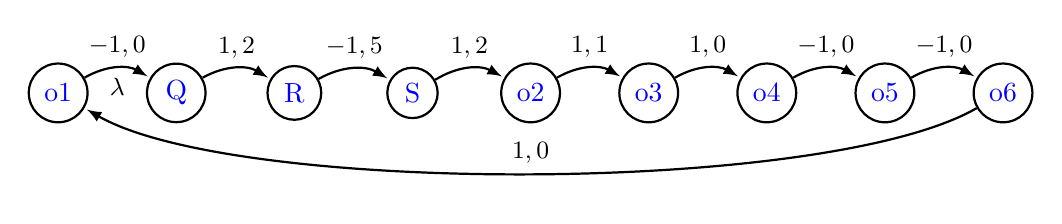
\begin{tikzpicture}[->,>=latex,shorten >=1pt,auto,node distance=1.5cm,
      thick,main node/.style={circle,draw}]
 \node[main node, fill=white, text=blue] (o1)  {o1};
 \node[main node, fill=white, text=blue] (Q) [right of=o1] {Q};
 \node[main node, fill=white, text=blue] (R) [right of=Q] {R};
 \node[main node, fill=white, text=blue] (S) [right of=R] {S};
 \node[main node, fill=white, text=blue] (o2) [right of=S] {o2};
 \node[main node, fill=white, text=blue] (o3) [right of=o2] {o3};
 \node[main node, fill=white, text=blue] (o4) [right of=o3] {o4};
 \node[main node, fill=white, text=blue] (o5) [right of=o4] {o5};
 \node[main node, fill=white, text=blue] (o6) [right of=o5] {o6};
 
\path[every node/.style={font=\sffamily\small}]
 (o1) edge [bend left] node [above] {$-1, 0$} node [below] {$\lambda$} (Q)
 (Q) edge [bend left] node [above] {$1, 2$} node [below] {} (R)
 (R) edge [bend left] node [above] {$-1, 5$} node [below] {} (S)
 (S) edge [bend left] node [above] {$1, 2$} node [below] {} (o2)
 (o2) edge [bend left] node [above] {$1, 1$} node [below] {} (o3)
 (o3) edge [bend left] node [above] {$1, 0$} node [below] {} (o4)
 (o4) edge [bend left] node [above] {$-1, 0$} node [below] {} (o5)
 (o5) edge [bend left] node [above] {$-1, 0$} node [below] {} (o6)
 (o6) edge [bend left, looseness=0.5] node [above] {$1, 0$} node [below] {} (o1)
 ;
\end{tikzpicture}

    \vskip -0.5cm
    \caption{In these electrocardiogram data, it is important for
      models (\textcolor{blue}{blue}) to accurately detect the QRS
      complex (Q is before the peak, R is the peak marked in
      \textcolor{red}{red}, S is the local minimum after the peak,
      other states o1--6). \textbf{Top:} Previous model of
      \citet{PanTompkins1985} mistakenly predicts S at the
      peak. \textbf{Middle:} proposed constrained change-point model
      accurately predicts R at each peak.  \textbf{Bottom:} graph
      structure of proposed nine-state constrained change-point model.
      Below each edge $e$ we show the penalty $\lambda_e$, which is
      either a constant $\lambda>0$ or zero if nothing is shown; above
      we show the constants $\delta_e,\gamma_e$ in the constraint
      function
      $g_e(m_i,m_{i+1})= \delta_e(m_i - m_{i+1})+\gamma_e\leq 0$
      ($\delta_e=1$ for a non-decreasing change, $\delta_e=-1$ for a
      non-increasing change, $\gamma_e \geq 0$ is the minimum
      magnitude of change).
      % source: https://github.com/tdhock/ecg-labels/blob/master/figure-one-ecg-graph.R
  }
\end{figure}

\bibliographystyle{abbrvnat}
\bibliography{refs}

\end{document}